% simple document template
\documentclass[12pt]{report}
\usepackage{tikz}
\usetikzlibrary{graphs}
\usetikzlibrary {mindmap}
\usetikzlibrary {positioning}
\usetikzlibrary {arrows.meta}
\usetikzlibrary {shapes.multipart}
\usetikzlibrary {shapes.geometric}
\usetikzlibrary {shapes.symbols}
\usetikzlibrary {shapes.callouts}
\usetikzlibrary {calc}
\begin{document}

\title{Notes for 2024}
\author{Pengfei Gao}

\maketitle

\tableofcontents

\section{LLM}

\section{Neural Network}
\subsection{Convolutional Neural Network}
\subsection{Attention Mechanism}
\subsubsection{2017-STRUCTURED ATTENTION NETWORKS}
% tags
\def \year{2017}
\def \refnum{597}
\def \pub{ICLR}
\begin{tikzpicture}[every node/.style={fill=orange!50!white, draw=gray!10!white, rounded corners=8, anchor=west}]
\node (a){\year}; 
\node (b) at (a.east) {\pub}; 
\node (c) at (b.east) {\refnum};
\end{tikzpicture}

% content synopse
\def \contribution{Explicitly introduce structure in to attention}
\def \usecase{QA, Text Summarization}
\def \thoughts{LLM is better than explicitly add structure into model}
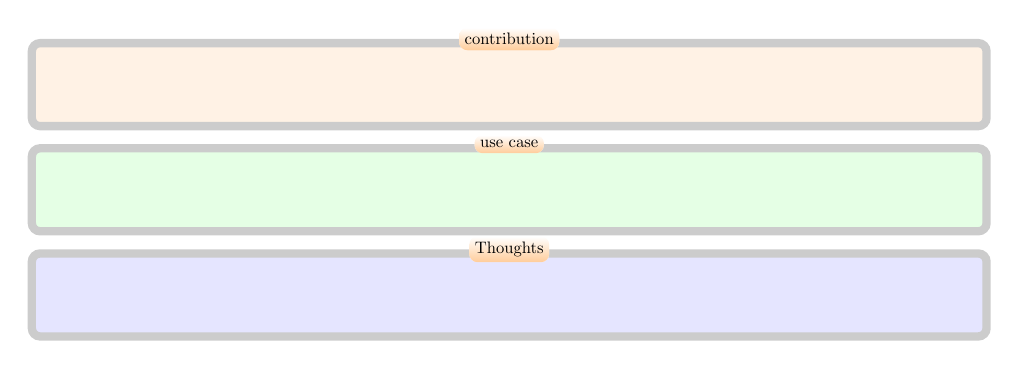
\begin{tikzpicture}[main/.style={
    fill=orange!10!white, 
    draw=gray!40!white,
    line width=3,
    minimum height=3em,
    minimum width=\textwidth,
    rounded corners=3, 
    align=left,
    anchor=north west},
    tag/.style={
        black, fill=white, bottom color=orange!40!white, top color=white, scale=0.6, rounded corners=3
    }
    ]
    \node[main] (a) {\contribution};
    \node[tag] at (a.north) {contribution};
    \node[main, fill=green!10!white] (b) at ($(a.south west) + (0, -0.5em)$){ \usecase};
    \node[tag] at (b.north) {use case};
    \node[main, fill=blue!10!white] (c) at ($(b.south west) + (0, -0.5em)$){ \thoughts};
    \node[tag] at (c.north) {Thoughts};
\end{tikzpicture}


\subsection{Transformer}

% =======传记=========
\section{biography}
\subsection{Hamilton}
\subsubsection{Who was Alexander Hamilton?}
% tags
\def \year{Pam Pollack}
\begin{tikzpicture}[every node/.style={fill=orange!50!white, draw=gray!10!white, rounded corners=8, anchor=west}]
\node (a){\year}; 
\end{tikzpicture}
% facts
\begin{verbatim}
Similar to the musical.
    * 1804: duel 
\end{verbatim}

\section{society}
\subsection{Squeezed: can not affort america}
\paragraph{Summary}~\\
This book is typical: complains about the system, no solution. Took survey in poor middle class with babies.

\end{document}